% politeness cogsci submission


\documentclass[10pt,letterpaper]{article}

\usepackage{cogsci}
\usepackage{pslatex}
\usepackage{color}
 \newcommand{\denote}[1]{\mbox{ $[\![ #1 ]\!]$}}
\usepackage[nodoi]{apacite}
\usepackage{graphicx}
\usepackage[american]{babel}
\usepackage{amsmath}
\usepackage{amssymb}
\usepackage[section]{placeins}
\usepackage{enumitem}
\usepackage{apacite}
\usepackage{url}
\usepackage{dblfloatfix}
 
\usepackage{caption}
\usepackage{subcaption}

 \definecolor{Red}{RGB}{255,0,0}
\newcommand{\red}[1]{\textcolor{Red}{#1}}
\definecolor{Green}{RGB}{10,200,100}
\definecolor{Blue}{RGB}{10,100,200}
\definecolor{DarkOrange}{RGB}{255,100,50}
\newcommand{\ndg}[1]{\textcolor{Green}{[ndg: #1]}}
\newcommand{\mht}[1]{\textcolor{DarkOrange}{[mht: #1]}}
\newcommand{\ejy}[1]{\textcolor{Blue}{[ejy: #1]}}
\newcommand{\mcf}[1]{\textcolor{Red}{[mcf: #1]}}

\title{Talking with tact: Polite language as a balance between kindness and informativity}

  \author{ {\large \bf Erica J. Yoon*}, {\large \bf Michael Henry Tessler*}, {\large \bf Noah D. Goodman}, and {\large \bf Michael C. Frank}   \\
\{ejyoon, mtessler, ngoodman, mcfrank\} @stanford.edu \\
  Department of Psychology, Stanford University \\
  *Authors contributed equally to this work.}


\begin{document}

\maketitle


\begin{abstract}

Conveying information in a false or indirect manner in consideration of listeners' wants (i.e. being polite)
seemingly contradicts an important goal of a cooperative speaker: information transfer.
We propose that a cooperative speaker considers both
\emph{epistemic utility}, or utility of providing the listener new and accurate information,
and \emph{social utility}, or utility of maintaining or boosting the listener's self-image (being polite).
We formalize this tradeoff within a probabilistic model of language understanding and test it with empirical data on people's inferences about the relation between a speaker's goals, utterances and the true states of the world.

\textbf{Keywords:}
Politeness; computational modeling; communicative goals; pragmatics

\end{abstract}


\section{Introduction}

Your friend gives a terrible presentation and asks for your opinion.
Must you admit, ``Your talk was terrible,'' or is it acceptable to say: ``Your talk was fine''?
The latter is potentially misleading but gives the listener what she might want to hear----in other words, it would be polite.

Politeness violates a critical principle of cooperative communication: exchanging information efficiently and accurately \cite{Grice1975}.
If information transfer was the only currency in communication, a cooperative speaker would find polite utterances undesirable because they are potentially misleading.
People are polite, however, and speakers do produce polite utterances.
Adults and even young children spontaneously produce requests in polite forms \cite{clark1980, axia1985}.
Speakers exhibit politeness strategies even while arguing, preventing unnecessary offense to their interactants \cite{holtgraves1997}.
Listeners even attribute ambiguous speech to a polite desire to hide a truth that could hurt another's self-image (e.g. \citeNP{bonnefon2009}).
In fact, it is difficult to imagine human speech that efficiently conveys only the truth.
Intuitively, politeness is one prominent characteristic that differentiates human speech from stereotyped robotic communication, 
which may try to follow rules to say ``please'' or ``thank you'' yet still lack genuine \emph{politeness}. 

Does this mean people are not cooperative communicators? 
\citeA{Brown1987} recast the notion of a \emph{cooperative speaker} as one
who has both an epistemic goal to improve the listener's knowledge state as well as a social goal to minimize any potential damage to the hearer's (and the speaker's own) self-image, which they called \emph{face}.
In their analysis, if the speaker's intended meaning contains no threat to the speaker or listener's face,
then the speaker will choose to convey the meaning in an efficient manner, putting it \emph{on the record}.
As the degree of face-threat becomes more severe, however,
a speaker will choose to be polite by producing more indirect utterances.

In the current paper, we formalize a version of \citeA{Brown1987}'s theory, exploring the idea that cooperative speakers attempt to balance two goals, epistemic and social.
The Rational Speech Act (RSA) framework \cite{Frank2012, Goodman2013} describes language understanding as recursive probabilistic inference between a pragmatic listener and an informative speaker. This framework has been successful at capturing the quantitative details of a number of language understanding tasks, but it neglects the social goals a speaker may pursue.
Here we extend RSA to take into account a speaker with both the usual epistemic goal and a competing social goal: be kind.
We test this model by gathering data about utterance interpretations and goal attributions in settings where the true state of the world carries affective consequences for the hearer.


\section{Computational Model}

Politeness poses a challenge for formal models of pragmatic language understanding, which assume that speakers' goals are to communicate informatively about some aspect of the world \cite{Frank2012, Goodman2013}.
RSA models a listener as reasoning about a speaker, who chooses utterances approximately optimally given a utility function.
\citeA{Goodman2013} define speaker utility by the amount of information a \emph{literal listener} would still not know about world state $s$ after hearing a speaker's utterance $w$ (i.e. \emph{surprisal}), what we will call \emph{epistemic utility}:
$U_{epistemic}(w; s) = \ln(P_{L_0}(s \mid w)) $,
where the literal listener is a simple Bayesian agent that takes the utterance to be true:
\begin{equation}
P_{L_0}(s \mid w)\propto \denote{w}(s) \cdot P(s) \label{eq:L0}.
\end{equation}
Here, $\denote{w}(s)$ is the truth-functional denotation of the utterance $w$ (i.e. the utterance's literal meaning): It is a function that maps world-states $s$ to Boolean truth values.
The literal meaning is used to update the literal listener's prior beliefs over world states $P(s)$.
%
\begin{figure*}[!b]
\begin{center}
  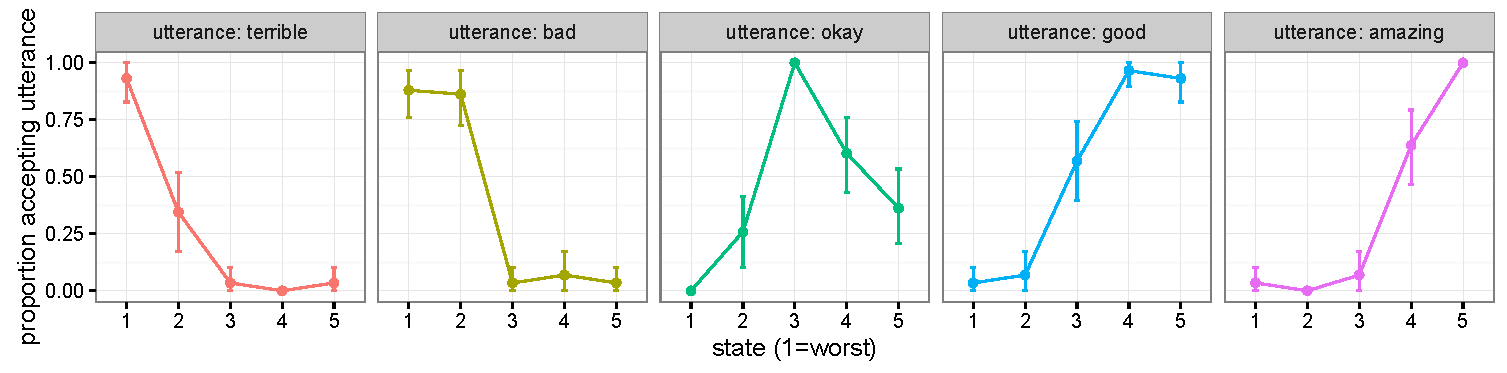
\includegraphics[width=.9\textwidth]{figures/exp1.pdf}
  \caption{\label{fig:exp1} Results from Experiment 1. Proportion of acceptances of words (shown in different colors) given the true state represented on a scale of hearts. Error bars represent 95\% confidence intervals.}
  \end{center}
\end{figure*}
%
%
%We propose that information transfer captures just one component of a speaker's utility, 
%Politeness then emerges from a second component of a speaker's utility, what we will call \emph{social utility}.

We propose there is a second component to the speaker's utility related to the intrinsic value of the state in the eyes of the listener\footnote{At this point, we do not differentiate state value to the listener from state value to the speaker, though in many situations these could in principle be different.}, what we will call \emph{social utility}.
%
We define the social utility of an utterance to be the expected utility of the state the listener would infer given the utterance $w$:
$$
U_{social}(w; s) = \mathbb{E}_{P_{L_0}(s \mid w)}[V(s)],
$$
%
where $V$ is a value function that maps states to subjective utility values---this captures the affective consequences for the listener of being in state $s$.
%
We take the overall speaker utility to be a weighted combination of epistemic and social utilities:
$$
U(w;s;  \hat{\beta}) = \beta_{epistemic}\cdot U_{epistemic} + \beta_{social} \cdot U_{social}.
$$
%
%
The speaker chooses utterances $w$ softmax-optimally (determined by \emph{speaker rationality} parameter $\lambda$) given the state $s$ and his goal weights $\hat{\beta}$: 
\begin{equation}
P_{S_1}(w \mid s, \hat{\beta}) \propto \mathrm{exp}(\lambda \cdot \mathbb{E}[U(w; s;  \hat{\beta})])\label{eq:S1}
\end{equation}
%
%Here we extend the speaker's utility by adding a component related to the intrinsic value of the state in the eyes of the listener.\footnote{At this point, we do not differentiate state value to the listener from state value to the speaker, though in many situations these could in principle be different.}
%
The pragmatic listener, denoted $L_1$, infers the world state based on this speaker model.
We will assume the listener does not know exactly how the speaker weights his competing goals, however.
Following the treatment of RSA using lifted variables \cite{GoodmanLassiter2015, bergen2016, Kao2014},
we assume the pragmatic listener jointly infers the state $s$ and the utility weights of the speaker, $\beta_{epistemic}$ and $\beta_{social}$:
\begin{equation}
P_{L_1}(s,  \hat{\beta} \mid w)\propto P_{S_1}(w \mid s,  \hat{\beta})\cdot P(s) \cdot P( \hat{\beta}) \label{eq:L1}
\end{equation}

Within our experimental domain, shown in Figure~\ref{fig:ex} and described in more detail below, we assume there are five possible states of the world corresponding to the value placed on a particular referent (e.g. the presentation the speaker is commenting on): $S = \{s_{1}, ...,  s_{5}\}$.
We further assume a uniform prior distribution over possible states of the world.
The states have subjective numerical values $V(s_{i}) = \alpha \cdot i$, where $\alpha$ is a scaling parameter (later inferred from data).
The set of utterances is \{\emph{terrible}, \emph{bad}, \emph{okay}, \emph{good}, and \emph{amazing}\}.
We implemented this model using the probabilisitic programming language WebPPL \cite{dippl} and a complete implementation can be found at \url{http://forestdb.org/models/politeness-cogsci2016.html}.

\begin{figure}[th]
\begin{centering}
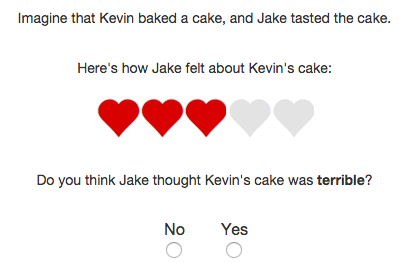
\includegraphics[width=3.2in]{figures/example.png}
\caption{\label{fig:ex} Example of a trial in Experiment 1.}
\end{centering}
\end{figure}


In what follows, we measure the literal semantics in Experiment 1, then use these to predict performance in two experiments. In Experiment 2, we explore listeners' inferences about the world $s$ given an utterance and a speaker's goal. In Experiment 3, we investigate inferences about speakers' goals given an utterance and a state. 
Then we compare the behavioral results to our model predictions, that people's inferences are based on a speaker model with two utilities, epistemic and social. 

\section{Experiment 1: Literal semantics}

\begin{figure*}[b]
\begin{centering}
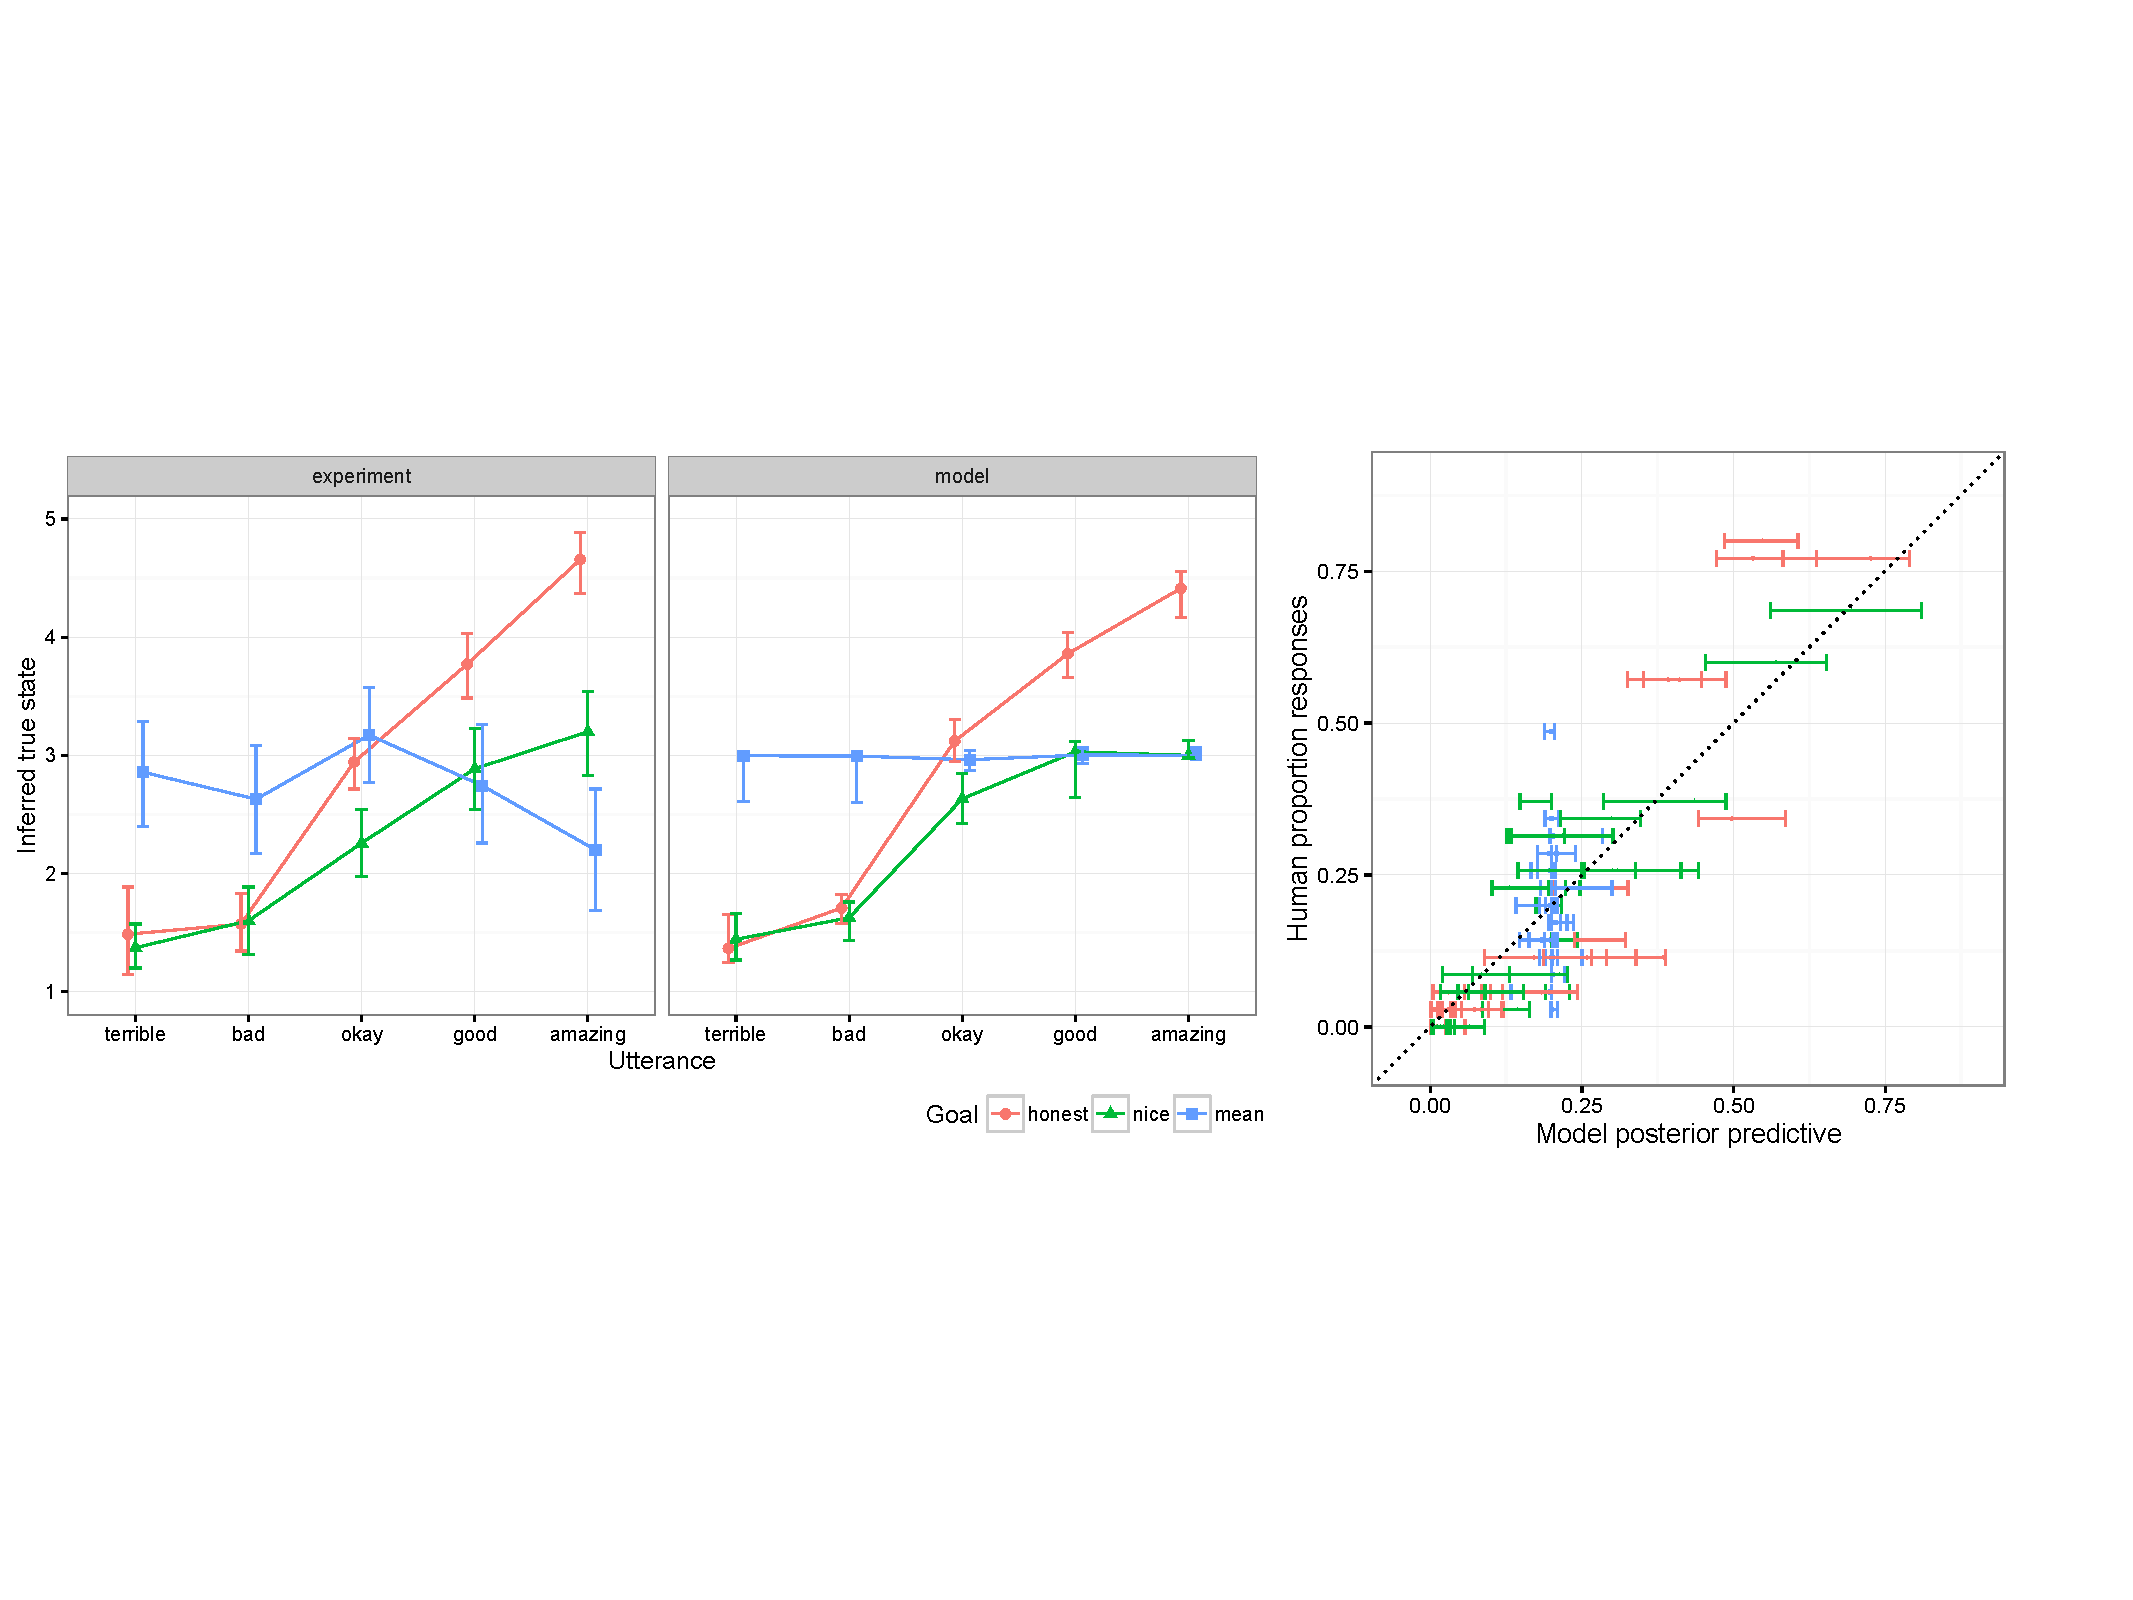
\includegraphics[width=\textwidth]{figures/exp2.pdf}
\caption{\label{fig:expt2} Results from Expt.~2 (left) and model predictions (center) for average states inferred based on a speaker's goal and utterance. Right: Full distribution of human responses vs. model predictions. Error bars represent 95\% confidence intervals for the data and 95\% highest density intervals for the model.}
\end{centering}
\end{figure*}

Experiment 1 measured judgments of literal meanings of our target words.
Responses in this experiment will be used to set expected literal meanings of words in our formal model.

\subsection{Method}

\noindent {\bf Participants}
30 participants with IP addresses in the United States were recruited on Amazon's Mechanical Turk.

\noindent {\bf Stimuli and Design}
We created 13 different context items, in which someone (e.g. Ann) gave a performance of some kind (e.g. gave a talk, performed a cello solo, baked a cookie, etc.), and another person (e.g. Bob) evaluated it. For example, in one of the contexts, Ann baked a cake, and Bob's true feelings toward Ann's cake (``\emph{true state}'') were shown on a scale out of five hearts. The question of interest was ``Do you think Bob thought Ann's cake was [\emph{terrible}, \emph{bad}, \emph{okay}, \emph{good}, or \emph{amazing}]?'' Each participant read 25 scenarios (5 true states and 5 words). 
The order of context items was randomized.

\noindent {\bf Procedure}
Participants read scenarios and indicated their answer to each question by answering `No' or `Yes' (see Figure~\ref{fig:ex} for a screenshot of an example trial).
The experiment can be viewed at: \url{http://langcog.stanford.edu/expts/EJY/polgrice/L2_J/polgrice_L2_J.html}.

\noindent {\bf Results}
In this and all subsequent experiments, we analyze the data by collapsing across contexts.
Meanings of the words as judged by participants were as one would expect (see Figure \ref{fig:exp1}).
Proportion of acceptances for a word given the true state peaked where the degree of positivity, neutrality and negativity of the state matched that of the word.
The fraction of participants that endorsed utterance $w$ for state $s$ will be used as the literal meaning $\denote{w}(s)$ in Eq. \ref{eq:L0}.

\section{Experiment 2: True state inference}

In Experiment 2, we examined listeners' inferences about the likely state of the world $s$ given a speaker's utterance (e.g. \emph{``It was good''}) and a description of the speaker's intentions (e.g. the speaker wanted to be \emph{nice}).

\subsection{Method}

\noindent {\bf Participants}
35 participants with IP addresses in the United States were recruited on Amazon's Mechanical Turk.


\noindent {\bf Stimuli and Design}
We designed scenarios in which a person (e.g. Ann) asked for another person (e.g. Bob)'s opinion on her performance. The same context items and true states as Experiment 1 were used. Additionally, we provided information on Bob's goal (to be \emph{honest}, \emph{nice}, or \emph{mean}) and what Bob actually said to Ann (e.g. ``It [your cake] was okay''), where Bob used one of the five possible words: \emph{terrible}, \emph{bad}, \emph{okay}, \emph{good}, or \emph{amazing}. Then we asked participants to infer the true state of the world (e.g. how Bob actually felt about Ann's cake). Each participant read 15 scenarios (3 goals and 5 words). The order of context items was randomized.

\noindent {\bf Procedure}
Participants read each story (e.g. Ann baked a cake and asked Bob about it) followed by a prompt that said,
e.g., ``Bob wanted to be nice: ``It was okay,'' he said. How do you think Bob actually felt about Ann's cake?''
Participants indicated their answer on a scale of five hearts. 
The experiment can be viewed at: \url{http://langcog.stanford.edu/expts/EJY/polgrice/L2_S/polgrice_L2_S.html}.

\subsection{Behavioral results}

Inferences of the actual rating for hearer's performance, or the true state, varied depending on speaker's goal and utterance (Figure \ref{fig:expt2}).
Consistent with intuition, when the speaker was trying to be honest, utterances accurately mapped onto inferred states (Figure \ref{fig:expt2}, left, red line).
For utterances consistent with the speaker's goals (e.g. saying positive utterances when the speaker was trying to be nice; negative utterances when trying to be mean), the results are also consistent with intuition.
Knowing that the speaker was trying to be nice, participants inferred a true state appreciably lower than the state inferred given honesty (green line).
The reverse was true when the speaker was trying to be mean (blue).


For utterances inconsistent with the speaker's goals, we observe an interesting asymmetry.
When the speaker was trying to be nice and said a negative utterance (e.g. ``it was bad''), participants inferred that the true state really was bad (no difference between an \emph{honest} ``bad'' and a \emph{nice} ``bad''), perhaps because of a floor effect or owing to the fact that one can be nice by being honest.
When the speaker was trying to be mean, however, and said a positive utterance (e.g. ``it was amazing''), participants inferred a state that is \emph{worse} compared to the states based on honesty and niceness goal.
This is likely due to participants attributing sarcasm or irony to the speaker who was trying to be mean.

\begin{figure}[!b] 
\begin{centering}
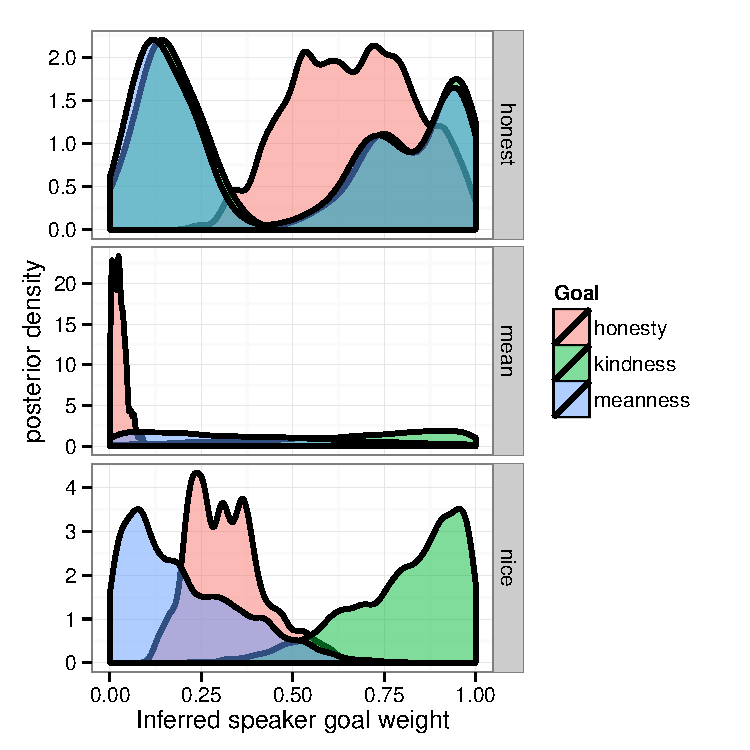
\includegraphics[width=0.70\columnwidth]{figures/goal-posterior.pdf}
\caption{\label{fig:goal-priors-bda} Inferred goal weights $\beta$ for Expt.~2.
Facets are different experimental conditions (trying to be X). 
Density plots show likely weights used in the speaker's utility function.
}
\end{centering}
\end{figure}


\subsection{Model predictions}

\noindent {\bf Model fitting}
In this experiment, participants were told the speaker said $w$ and described what the speakers' intentions were (e.g. \emph{Bob wanted to be nice}).
We want to explore inferences both when speaker wanted to be nice and when he wanted to be mean: For ease of comparison to the experimental data, we assume each $\beta \in [0,1]$ and separate $\beta_{social}$ into a positive component ($\beta_{nice}$) and a negative component ($\beta_{mean}$), writing the utility function now as
$$
 U(w;s; \beta)  =  \beta_{epistemic}\cdot U_{epistemic} + (\beta_{nice} - \beta_{mean}) \cdot U_{social}
 $$
We assume that the intentions (e.g. \emph{wanted to be nice}) notified the listener of a particular set of goal-weights \{$\beta_{nice}, \beta_{honest}, \beta_{mean}$\} that the speaker was using.
We put uninformative priors on these weights ($\beta \sim \text{Uniform}(0,1)$) and infer their credible values separately for each goal condition (``trying to be X'') using Bayesian data analytic techniques \cite{LW2014}.

There are 2 additional parameters of the cognitive model: the speaker optimality parameter $\lambda$ in Eq.~\ref{eq:S1} and the value scale parameter $\alpha$ in the utility function.
We put uninformative priors on these ($\lambda \sim \text{Uniform}(0,20)$ and $\alpha \sim \text{Uniform}(0, 5)$) and infer their posterior credible values from the data.
We ran 2 MCMC chains for 100,000 iterations, discarding the first 50,000 for burnin.
The Maximum A-Posteriori (MAP) estimate and 95\% Highest Probability Density Interval (HDI) for $\lambda$ is 1.8 [1.08, 3.1]; for $\alpha$ is 9.1 [3.4, 9.9]. %; for $\phi$ is \red{0.09 [0.06, 0.13]}.
To generate predictions, given our cognitive model and the inferred parameters, we evaluated the posterior predictive distribution, marginalizing out all parameters.

\noindent {\bf Results}
The inferred weights for each goal condition were largely as expected (Figure~\ref{fig:goal-priors-bda}).
For the ``trying to be honest'' condition, the model infers the speaker was using a non-zero weight on honesty, while the overall social weight is zero (since niceness and meanness are inferred to be the same values and they inverses of each other).
For ``trying to be nice'', the model puts a high weight on niceness but also some appreciable weight on honesty.
The model fits are worse for the ``trying to be mean'' case; all that the model infers is that the speaker was not honest.

The predictions of the expectations of the listener model for the \emph{true state} (Eq.~\ref{eq:L1}) are shown in Figure \ref{fig:expt2} (center).
The model's expected posterior over states when the speaker is trying to be \emph{honest} increases as a function of the positivity implied by the utterances (e.g. ``amazing'' means a very high state).
When it knows the speaker was trying to be \emph{nice}, the pragmatic listener is more conservative in how it interprets positive utterances, with the difference between an honest utterance and a nice utterance increasing as the utterance becomes more positive. 
For example, the difference between a \emph{nice} ``amazing'' and an \emph{honest} ``amazing'' is greater than the difference between a \emph{nice} ``okay'' and an \emph{honest} ``okay''.
Inferences when the speaker is trying to be \emph{mean} display the associated opposite behavior when the utterance is indeed negative (e.g. ``terrible'').
Overall, the expected values of the model explain a lot of the variance in the average data $r^2(15) = 0.91$.
The main discrepancies are with the goal ``trying to be mean'', as noted above.
Among the other 2 goal conditions, the model explains almost all of the variance $r^2(10) = 0.97$.

The model makes predictions not only for the average data but also for the full distribution of responses (Figure \ref{fig:expt2}, right).
The model predicts the full distribution with relatively high accuracy $r^2(75) = 0.79$.
% predictive accuracy is even higher for just the goals to be honest and nice $r^2(50) = 0.86$.

In sum, the model captured key aspects of our empirical findings.
The largest discrepancies appear in the experimental condition of the goal to be mean.
Participants thought that a mean speaker saying ``[your cake] was amazing'' meant the true state was below average, which the model was unable to accommodate.
This deviation is likely due to the effect of irony: making an extremely positive remark about an extremely bad performance is perceived to be sarcastic and ill-intentioned \cite{colston1997}.
Our model does not include sarcastic interpretation though other models in the RSA family do \cite{Kao2015}, and future work should address the delicate interplay of politeness and sarcasm.

\section{Experiment 3: Goal inference}

\begin{figure*}[!t]
\begin{center}
  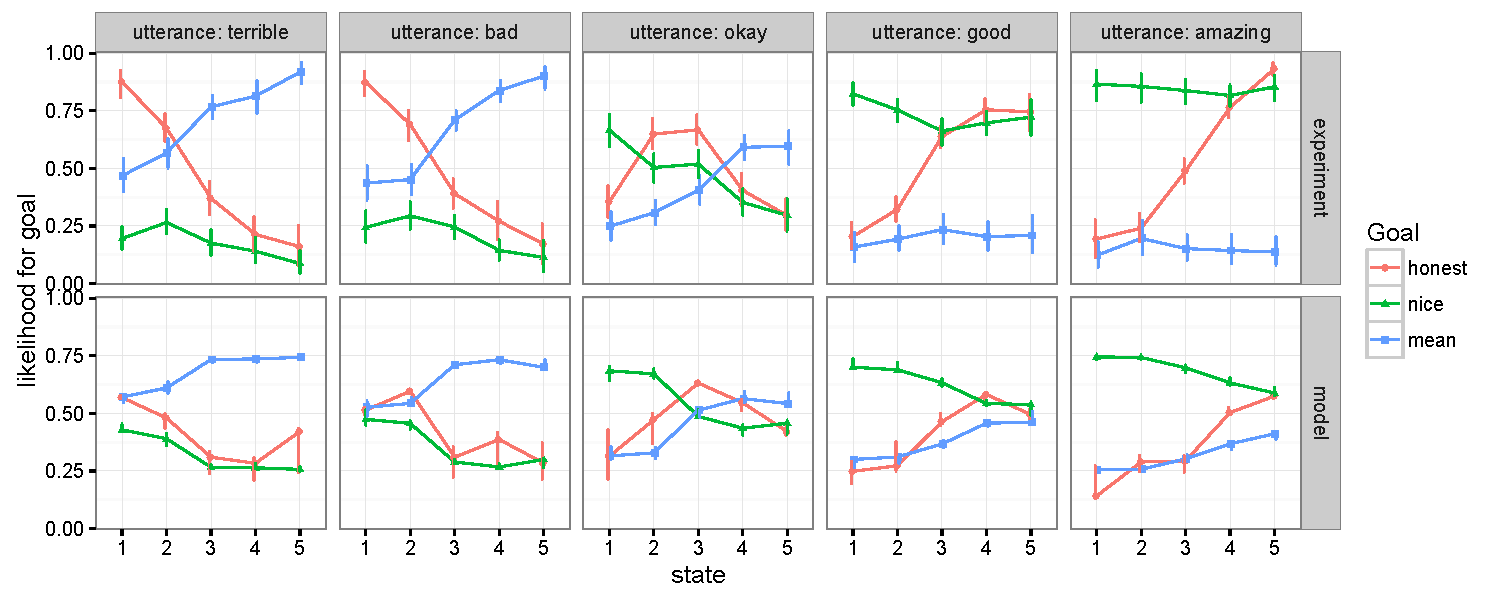
\includegraphics[width=\textwidth]{figures/exp3.pdf}
  \caption{\label{fig:expt3} Results from Expt.~3 (top) and model predictions (bottom). Attribution of speaker's goals: honest, nice and mean (colors) based on the true state and utterance. Error bars represent 95\% CIs for the data and 95\% HDIs for the model.}
  \end{center}
\end{figure*}

Experiment 3 probed listeners' inferences of the speaker's goals, given an utterance (e.g. \emph{``It was good''}) and a true state (e.g. 2 out of 5 hearts).

\subsection{Method}

\noindent {\bf Participants}
45 participants with IP addresses in the United States were recruited on Amazon's Mechanical Turk.


\noindent {\bf Stimuli and Design}
We presented the same context items and utterances as Experiment 2.
But instead of goals, we provided information on the true states (i.e. how Bob actually felt towards Ann's performance).
Then we asked participants to infer the likelihood of Bob's goals to be \emph{honest}, \emph{nice}, and \emph{mean}.
Each participant read 25 scenarios (5 true states and 5 words).
The order of context items was randomized.

\noindent {\bf Procedure}
Participants read each scenario followed by a question that read, ``Based on what Bob said, how likely do you think that Bob's goal was to be: honest; nice; mean,'' with the three goals placed in a random order below three slider bars, on which the participant could indicate each goal's likelihood. 
The experiment can be viewed at: \url{http://langcog.stanford.edu/expts/EJY/polgrice/L2_G/polgrice_L2_G.html}.



\subsection{Behavioral results}

Participants rated speaker's goals differentially depending on the true state and utterance (see Figure \ref{fig:expt3}, top).
Honesty was rated highest when the true state was most consistent with the literal semantics. 
As utterances became more positive, participants rated the speaker's niceness higher and meanness displayed the reverse pattern. 
Ratings for niceness and meanness goals were strongly anti-correlated $r = -.78$.

Interestingly, we observe an asymmetry in how positive and negative utterances map onto the goals of niceness and meanness, respectively. 
Participants reported that \emph{truthfully} saying ``amazing'' is both honest and nice, while \emph{truthfully} saying something is ``terrible'' is honest and not that mean.
Here, meanness can decrease in likelihood (i.e. be \emph{explained away}) because of honesty.
And yet honesty does not explain away niceness when the speaker says a truthful ``amazing''. 
%To our knowledge, this is the first evidence of an asymmetry in honesty can \emph{explain away} social goals.

\subsection{Model predictions}

\noindent {\bf Model fitting}
The model in Eq.~\ref{eq:L1} specifies a joint-belief distribution over the speaker's goals $\beta$ and possible states of the world $s$.
To compare to the empirical data, we condition on the true state of the world given in the experimental condition, and compare the marginal distribution of the speaker's goals $\beta$ to the empirical ratings.
We separate $\beta_{social}$ into  $\beta_{nice}$ and  $\beta_{mean}$, as in Expt.~2.
With no prior knowledge about the speaker's intentions, we assume a uniform prior over the goal-weights in the speaker's utility function: $\beta \sim \text{Uniform}(0,1)$.

We put the same priors over the speaker optimality parameter $\lambda$ and the value scale parameter $\alpha$.
We ran 2 MCMC chains for 40,000 iterations, discarding the first 20,000 for burnin.
The MAP estimate and 95\% HDI for $\lambda$ is 4.6 [4.0, 4.9]; for $\alpha$ is 1.17 [1.04, 1.31].%; for $\phi$ is 0.09 [0.06, 0.13].
%This is a relatively low value for $\phi$: The model explains about 90\% of the data set better than a model of random guessing.

\noindent {\bf Results}
The predictions of the model are shown in Figure~\ref{fig:expt3} (bottom).
Like our participants, the model believes the speaker to be more honest when the utterance matches the true state of the world, as given by the literal semantics data (Figure~\ref{fig:expt3}, red lines).
Further, the model increases its ratings of niceness as the utterance better matches states with higher values (green lines, main effect of panel).
The goal to be mean displays the opposite behavior, increasing as the utterance matches states with lower values (blue lines).
Overall, the model displays a strong quantitative fit to the goal inference data $r^2(75) = 0.87$.

The model successfully captured the key patterns in the data:
changing goal likelihoods based on the degree of match, and positivity/negativity bias of mismatch, between the utterance and true state.
The biggest mismatch seems to be that the model under-predicts the goal to be honest for every utterance except \emph{okay}.
This may be because explicitly positive/negative utterances can also be explained by a social goal in the model.
The model also does not capture the interaction that a truthful positive utterance is both honest and nice, while a truthful negative utterance is honest and not that mean.
 The model treats niceness and meanness as perfectly opposite to each other, while there is an interesting asymmetry in participants' behavior. 
This asymmetry may be because listeners expect honesty and niceness to be correlated \emph{a priori}, and anti-correlated with meanness, rather than independent as assumed by the model.

\section{Discussion}

Why would a speaker ever say something that is not maximally truthful and informative?
Communication is often examined from the perspective of successful information transfer from speaker to listener.
In the social realm, however, communication also can serve the social function of making the listener feel good and saving her face.

We proposed here that intuitively ``polite'' utterances arise from the desire to be kind (i.e. save face). 
A cooperative speaker then tries to balance the goals to be kind and to be informative, and produces utterances of varying degrees of politeness that reflect this balance.
To test this proposal, we examined inferential judgments on a speaker's utterance, which was a potentially face-threatening evaluation of the listener's performance.
As we predicted, participants' inferences about the true state of the world differed based on what the speaker said and whether the speaker's intended goal was to be honest, nice or mean (Expt.~2).
We were also able to predict participants' attributions of different social goals to speakers depending on
how well the literal utterance meaning matched the actual rating the performance deserved (Expt.~3).

The model presented here relates to other work done in game-theoretic pragmatics.
\citeA{VanRooy2003} uses a game-theoretic analysis of polite requests (``Could you possibly take me home?'') to argue the purpose of polite language is to align the preferences of interlocutors. 
Our notion of social utility $U_{social}$ is similar in that it motivates speakers to signal worlds that make the listener feel good. 
\citeauthor{VanRooy2003}'s analysis, however, relies on the notion that polite language is \emph{costly} (in a social way e.g., by reducing one's social status or incurring social debt to one's conversational partner) but it's not clear how the polite behaviors explored in our experiments (not polite requests) would incur any cost to speaker or listener. 
Our model derives its predictions by construing the speaker utility as a collection of possible goals (here, epistemic and social goals). The speech-acts themselves are not costly. 



Will machines ever be polite?
Politeness requires more than merely saying conventionalized words (\emph{please}, \emph{thank you}) at the right moments; it requires a balance of informativity and kindness.
Politeness is not an exception to rational communication; it is what makes human communication rational, by serving a key social function of maintaining relationships.
We extended the Rational Speech Acts framework to include social utility as a motive for utterance production.
This work takes a concrete step toward quantitative models of the nuances of polite speech.
And it moves us closer to courteous computation---to computers that communicate with tact.

\section{Acknowledgments}

This work was supported by NSF grant BCS \#1456077 and ONR grant N00014-13-1-0788. 

\bibliographystyle{apacite}
\setlength{\bibleftmargin}{.125in}
\setlength{\bibindent}{-\bibleftmargin}

\bibliography{politeness}

\end{document} 